\documentclass[journal,12pt,twocolumn]{IEEEtran}
\usepackage{tikz}
\usepackage{amsmath}
\usepackage{breqn}
\usepackage{amssymb}
\pagestyle{empty}
\usepackage{setspace}
\usepackage{gensymb}
\singlespacing

\usepackage{amsmath}
\usepackage{amsthm}
\begin{document}
\newcommand{\myvec}[1]{\ensuremath{\begin{pmatrix}#1\end{pmatrix}}}
\newcommand{\cmyvec}[1]{\ensuremath{\begin{pmatrix*}[c]#1\end{pmatrix*}}}
\providecommand{\norm}[1]{\lVert#1\rVert}
\newcommand{\mydet}[1]{\ensuremath{\begin{vmatrix}#1\end{vmatrix}}}
\providecommand{\sbrak}[1]{\ensuremath{{}\left[#1\right]}}
\providecommand{\lsbrak}[1]{\ensuremath{{}\left[#1\right.}}
\providecommand{\rsbrak}[1]{\ensuremath{{}\left.#1\right]}}
\providecommand{\brak}[1]{\ensuremath{\left(#1\right)}}
\providecommand{\lbrak}[1]{\ensuremath{\left(#1\right.}}
\providecommand{\rbrak}[1]{\ensuremath{\left.#1\right)}}
\providecommand{\cbrak}[1]{\ensuremath{\left\{#1\right\}}}
\providecommand{\lcbrak}[1]{\ensuremath{\left\{#1\right.}}
\providecommand{\rcbrak}[1]{\ensuremath{\left.#1\right\}}}
\let\StandardTheFigure\thefigure
\let\vec\mathbf

\title{
Assignment - 2
}
\author{ Soham Bhatt \\SM21MTECH14004}
\maketitle
\newpage
\bigskip
\bibliographystyle{IEEEtran}
\section*{\textbf{Problem}}
\noindent
\textbf{\textsl{1. Find the in-center of the triangle formed by the following points lie,}}
$$$$
\textbf{\textsl{i. 5x-12y=0,\quad ii. 5x+12y+60=0,\quad iii. 5x+12y-60=0}}
\noindent
\section*{\textbf{Solution}}
\noindent
First, we need to find the intersection point of given three lines, \\
\\
Let's find the intersection of line (i) and (ii),\\
\\
Let's write it vector form,
\begin{align*}
\vec{A}\vec{M} &=\vec{B} \\
\vec{M} &= \vec{A}^{-1}\vec{B} \\
\vec{M}
& =
\begin{bmatrix}
5 & -12 \\
5 & 12 
\end{bmatrix}^{-1}
\begin{bmatrix}
0 \\ -60
\end{bmatrix}  \\[6pt]
\vec{M}
& =
\frac{1}{120}
\begin{bmatrix}
12 & 12 \\
-5 & 5 
\end{bmatrix}
\begin{bmatrix}
0 \\ -60
\end{bmatrix} \\[6pt]
\vec{M}
&=
\begin{bmatrix}
-6 \\ -2.5
\end{bmatrix}
\end{align*}
In the same way, intersection of line (ii) and (iii) is,
\begin{align*}
\vec{A}\vec{N} &=\vec{B} \\
\vec{N} &= \vec{A}^{-1}\vec{B} \\
\vec{N}
& =
\begin{bmatrix}
5 & 12 \\
12 & 5 
\end{bmatrix}^{-1}
\begin{bmatrix}
-60 \\ 60
\end{bmatrix}  \\[6pt]
\vec{N}
& =
\frac{1}{119}
\begin{bmatrix}
5 & -12 \\
-12 & 5 
\end{bmatrix}
\begin{bmatrix}
-60 \\ 60
\end{bmatrix} \\[6pt]
\vec{N}
&=
\begin{bmatrix}
8.571 \\ -8.571
\end{bmatrix}
\end{align*}
In the same way, intersection of line (i) and (iii) is,
\begin{align*}
\vec{A}\vec{O} &=\vec{B} \\
\vec{O} &= \vec{A}^{-1}\vec{B} \\
\vec{O}
& =
\begin{bmatrix}
5 & -12 \\
12 & -5 
\end{bmatrix}^{-1}
\begin{bmatrix}
0 \\ 60
\end{bmatrix}  \\[6pt]
\vec{O}
& =
\frac{1}{169}
\begin{bmatrix}
-5 & 12 \\
-12 & 5 
\end{bmatrix}
\begin{bmatrix}
0 \\ 60
\end{bmatrix} \\[6pt]
\vec{O}
&=
\begin{bmatrix}
4.260 \\ 1.775
\end{bmatrix}
\end{align*}\\ \\
Now we need to find difference between each vectors,\\
Difference between vectors N and O:\\ \\
\vec{N} = \myvec{8.571\\-8.571}, O = \myvec{4.260\\1.775}\\ \\
\vec{0-N} = \myvec{-4.311\\10.345}\\
\begin{align*}
\norm{\vec{O}-\vec{N}}^2 &= (\vec{O}-\vec{N})^\top (\vec{O}-\vec{N})\\ \nonumber
\norm{\vec{O}-\vec{N}}&=\myvec{-4.311 \ 10.345} \myvec{-4.311\\10.345}\\ \nonumber
\norm{\vec{O}-\vec{N}}&=\sqrt{(-4.311^2 + 10.345^2)}\\ \nonumber
\norm{\vec{O}-\vec{N}}&=11.207 \qquad\qquad (\vec{D_1})\\ \nonumber
\end{align*}
Difference between vectors M and O:\\ \\
M = \myvec{-6\\-2.5}, O = \myvec{4.260\\1.775}\\ \\
0-M = \myvec{10.260\\4.275}\\
\begin{align*}
\norm{\vec{O}-\vec{M}}^2 &= (\vec{O}-\vec{M})^\top (\vec{O}-\vec{M})\\ \nonumber
\norm{\vec{O}-\vec{M}}&=\myvec{10.260 \ 4.275} \myvec{10.260\\4.275}\\ \nonumber
\norm{\vec{O}-\vec{M}}&=\sqrt{(10.260^2 + 4.275^2)}\\ \nonumber
\norm{\vec{O}-\vec{M}}&=11.115 \qquad\qquad (\vec{D_2}) \\\nonumber
\end{align*}
Difference between vectors M and N:\\ \\
M = \myvec{-6\\-2.5}, N = \myvec{8.571\\-8.571}\\ \\
N-M = \myvec{14.571\\-6.071}\\
\begin{align*}
\norm{\vec{N}-\vec{M}}^2 &= (\vec{N}-\vec{M})^\top (\vec{N}-\vec{M})\\ \nonumber
\norm{\vec{N}-\vec{M}}&=\myvec{14.571 \ 6.071} \myvec{14.571\\6.071}\\ \nonumber
\norm{\vec{N}-\vec{M}}&=\sqrt{(14.571^2 + 6.071^2)}\\ \nonumber
\norm{\vec{N}-\vec{M}}&=15.785 \qquad\qquad (\vec{D_3}) \\ \\\nonumber
\end{align*}
Formula for finding in-center (I) of triangle with three given coordinates is,\\
$$ \bigg(\frac{D_1M + D_2N + D_3O}{D_1+D_2+D_3} ,\quad\frac{D_1M + D_2N + D_3O}{D_1+D_2+D_3}\bigg) $$
\\
By putting all the values,\\
$$ \bigg(\frac{(11.207)(-6) + (11.115)(8.571) + (15.785)(4.260)}{11.207+11.115+15.785} ,$$
$$\quad\frac{(11.207)(-2.5) + (11.115)(-8.571) + (15.785)(1.775)}{11.207+11.115+15.785}\bigg) $$
\\ \\
\vec{I} = \myvec{2.500\\-2.499}

\begin{figure}
    
    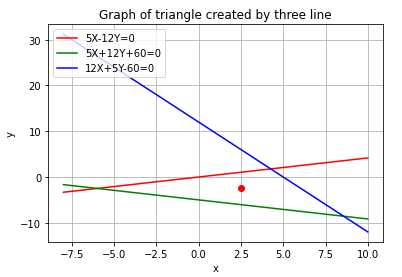
\includegraphics[width=\columnwidth]{graph.png}
    \caption{Triangle created by three lines}
    \label{fig:assignment-2}
\end{figure}

\end{document}